\documentclass{letask}

\begin{document}
\begin{titlepage}
\center % Center everything on the page
 
%----------------------------------------------------------------------------------------
%	HEADING SECTIONS
%----------------------------------------------------------------------------------------

\textsc{\LARGE Московский\\[-0.2cm]Физико-Технический Институт\\[0.1cm]\large (государственный университет)}\\[1.5cm] % Name of your university/college
\textsc{\Large Кафедра общей физики}\\[0.1cm] % Major heading such as course name
\textsc{\large Лабораторная работа \textnumero  4.4.1}\\[0.5cm] % Minor heading such as course title

%----------------------------------------------------------------------------------------
%	TITLE SECTION
%----------------------------------------------------------------------------------------

\HRule
\\[0.4cm]
{ \huge \bfseries Амплитудная\\[0.2cm]
дифракционная решетка}
\\[0.6cm] % Title of your document
\HRule
\\[1.5cm]


 
%----------------------------------------------------------------------------------------
%	AUTHOR SECTION
%----------------------------------------------------------------------------------------

\begin{minipage}{0.4\textwidth}
	\begin{flushleft} \large
		\textsf{Студент}
		
		Ришат \textsc{Исхаков} \\[-0.15cm]
		513 группа
	\end{flushleft}
\end{minipage}
~
\begin{minipage}{0.4\textwidth}
	\begin{flushright} \large
		\textsf{Преподаватель}
		
		Александр Александрович \\[-0.15cm]
		\textsc{Казимиров} % Supervisor's Name
	\end{flushright}
\end{minipage}

\begin{bottompar}
	\begin{center}
		
\includegraphics[width = 80 mm]{logo.jpg}
	\end{center}
	{\large \today}

\end{bottompar}
\vfill % Fill the rest of the page with whitespace

\end{titlepage}

\textbf{Цель работы:}
изучение свойства голограмм точечного источника и объемного предмета.
\textbf{В работе используются:} гелий-неоновый лазер, голограммы, набор линз, экран, линейка.

\section{Теоретическая часть}

\subsection*{Голограмма точки}
\begin{wrapfigure}[10]{r}{8.5 cm}
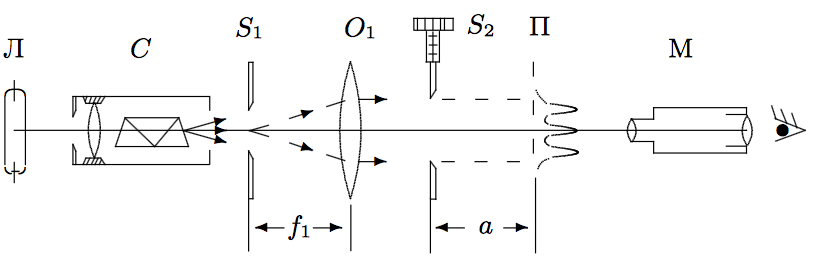
\includegraphics[width = 8 cm]{img1}
\caption{Запись голограммы точки}
\end{wrapfigure}
Обычная картина распределения интенсивности света не полностью характеризует световое поле -- информация о его фазе остается утерянной. Метод \textsf{восстановления волнового фронта} состоит в том, что на фотопластинке фиксируется интерференционная картина предметной и \textsf{опорной} волн. Обе волны должны быть когерентными, иначе не будет интерференции. Интенсивность такого светового возмущения несет информацию не только об амплитуде, но и о фазе рассеянной волны. Такая интерферограмма называется \textsf{голограммой}. Если затем осветить голограмму опорной волной, возникнет объемное изображение объекта.

Интерферометр Фабри-Перо состоит из двух отражающих пластин, внутренние поверхности которых хорошо отполированы и установлены параллельно друг другу. Его можно рассматривать как плоскопараллельную воздушную пластину, на которой происходят многократные отражения и интерференция световых лучей. Интерференционная картина, наблюдаемая в фокальной плоскости линзы Л, состоит из концентрических колец. 
Для двух соседних лучей, распространяющихся между зеркалами интерферометра под углом $\theta$, разность хода определяется соотношением
 
\begin{equation}
\Delta = 2 L \cos \theta,
\label{eq:dif}
\end{equation}

где $L$~--~расстояние между зеркалами интерферометра.
Будем считать, что поглощение света в зеркалах отсутствует, что достигается лишь при целых значениях отношения $\Delta / \lambda$.

Интерференционная картина состоит из узких светлых колец, разделенных широкими промежутками, расстояния между которыми мы будем измерять.

\section{Установка и параметры измерения}

\subsection{Определение цены деления}
Включим лазер и определим цену деления предметной шкалы. Осветим шкалу и получим \textsf{четкую} дифракционную картину. 

Цену деления рассчитаем по формуле для дифракции Фраунгофера: 
\[ D = \dfrac{\lambda}{\Delta x}, \] 
где $\Delta x$~--~расстояние между дифракционными максимумами, $L$~--~расстояние от шкалы от экрана.
\[\Delta x = 2 \cm, \quad L = 107 \cm, \quad \lambda = 532 \nm, \]
тогда $D = (1.13 \pm 0.03) \cdot 10^{-4} \; \cm$~--~цена деления предметной шкалы.

Определим цену деления вторым методом, установив линзу с фокусным расстоянием $F~\approx~4 \;\cm$ и получим в центре экрана увеличенное изображение предметной шкалы с четкими делениями.

Измерим расстояния от линзы до предметной шкалы $a$ и до экрана $b$ и рассчитаем увеличение системы. Определите расстояние $D$ между изображениями штрихов и рассчитаем цену деления D предметной шкалы:
\[\Delta x = 0.23 \; \cm, \quad a = 4.5 \; \cm, \quad b = 102.5 \; \cm, \]
\[D = \dfrac{\Delta x}{\Gamma} = (1.11 \pm 0.05) \]

\subsection{Точечный источник}

Получаем на экране изображение голограммы точечного источника -- наиболее четкое изображение колец. 
Измерим радиусы нескольких темных колец.

\begin{table}[H]
\centering
\begin{tabular}{|c|c|c|c|c|}
\hline
n & $r, \mm$ & $r_\text{гол}$ & $\Delta r, \mm$ & $d, \mm$ \\ \hline
1 & 3        & 0.13           & 0.01            & 38.12    \\ \hline
2 & 4        & 0.18           & 0.01            & 41.11    \\ \hline
3 & 6        & 0.27           & 0.02            & 39.55    \\ \hline
4 & 7        & 0.31           & 0.02            & 39.9    \\ \hline
5 & 8        & 0.36           & 0.02            & 38.37    \\ \hline
\end{tabular}
\caption{Радиусы темных колец и расстояния до источника при создании голограммы}
\end{table}

Тогда $\overline{d} = (39.5 \pm 5.2) \; \mm$

Перемещая линзу вдоль луча, получаем на экране изображение сначала мнимого $O_2$, затем действительного источника $O_3$.
Измерив полученные размеры, посчитаем расстояние от точечного источника до голограммы.

Расстояние от линзы до $O_2 = (105.1 \pm 0.5 ) \; \cm$

Расстояние от линзы до $O_3 = (98.2 \pm 0.5 ) \; \cm$

Тогда расстояние от точечного источника до голограммы $O_2 = (4.36 \pm 0.04) \; \cm$

Тогда расстояние от точечного источника до голограммы $O_3 = (4.32 \pm 0.04) \; \cm$

\subsection{Изучение фокусирующих свойств голограммы}
Добиваемся полного разделения пучков света на экране и определяем, какой из них соответствует действительному, какой мнимому изображению. 

Установив перед голограммой предметную шкалу, получаем четкое изображение шкалы в пятне, соответствующем действительному изображению.

Измерьте расстояние между штрихами $D'$ на экране и расстояние $b$ от экрана до голограммы. Используя эти данные, а также найденную ранее цену деления шкалы $D$, рассчитаем фокусное расстояние голографической линзы.

\[ D' = (0.35 \pm 0.01) \; \cm/\text{дел}; \quad b = (123.4 \pm 1) \; \cm) \]
\[ F = \dfrac{b}{1+\frac{D}{D'}} = (3.8 \pm 0.1) \; \cm \]

\subsection{Изучение характеристик голограммы объемного предмета}

Настроив систему и получив голограмму в расширенный пучок лазера находим мнимое изображение предмета. 
$ \alpha = 32^o \pm 2^o $~--~угол поворота голограммы, то есть такой же угол падения опорного пучка.

Постепенно закрываем голограмму листом бумаги и видим, что изображение почти не меняется, то есть восстанавливается не из полной картины.

На мнимом изображении видим линейку, а за ней стержень. На действительном изображении картина обратная, то есть стержень расположен перед линейкой. Попробуем оценить расстояние от стержня до линейки.

Для этого рассмотрим отметку на линейке при разных углах поворота:

\begin{figure}[H]
\centering
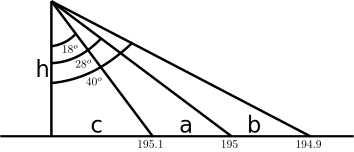
\includegraphics[width = 0.6 \lw]{drawing}
\caption{Расчет расстояния между линейкой и стержнем}
\end{figure}

\begin{equation}
\begin{cases}
\tg 18^o = \dfrac{c}{h} \\
\tg 28^o = \dfrac{c+a}{h} \\
\tg 40^o = \dfrac{c+a+b}{g} \\
\end{cases}
\quad \Rightarrow \quad
h = \dfrac{a+b}{\tg 40^o - \tg 18^o} = \dfrac{a}{\tg 28^o - \tg 18^o} = \dfrac{b}{\tg 40^o - \tg 28^o} 
\end{equation}
\[h = (0.39 \pm 0.07) \; \cm \]


\subsection{Изучение действительного изображения}

Находим действительное изображение, поворачиваем голограмму на $180^o$ вокруг вертикальной оси.

Угол падения восстанавливающей волны, при которых возникает действительное изображение~--~$30^o$, мнимое изображение~--~$24^o$.

Снова разворачиваем голограмму эмульсией к лазеру. Перемещаем короткофокусную линзу расширителя вдоль луча, наблюдаем, что при приближении линзы к лазеру изображение действительное увеличивается, мнимое уменьшается.

\section{Вывод}
Мы собственноручно восстановили голограмму сначала точечного источника, затем объемного предмета и оценили расстояния, с которых создавалась голограмма. Убедились в том, что частичное перекрытие светового потока слабо влияет на полученное в результате изображение.

\end{document}
